\documentclass[11pt]{beamer}
\usepackage[utf8]{inputenc}
\usepackage[T1]{fontenc}
\usepackage{lmodern}
\usetheme{AnnArbor}
\usepackage{graphicx}
\usepackage{amsmath}
\begin{document}
	\author{Manosh}
	\title{First PPT L for \LaTeX}
	\subtitle{India}
	%\logo{}
	\institute{IIT}
	\date{\today}
	\subject{Physics}
	%\setbeamercovered{transparent}
	%\setbeamertemplate{navigation symbols}{}
	\begin{frame}[plain]
		\maketitle
	\end{frame}
	
	\begin{frame}
		\frametitle{Intro}
	\end{frame}

\begin{frame}
	\begin{figure}
		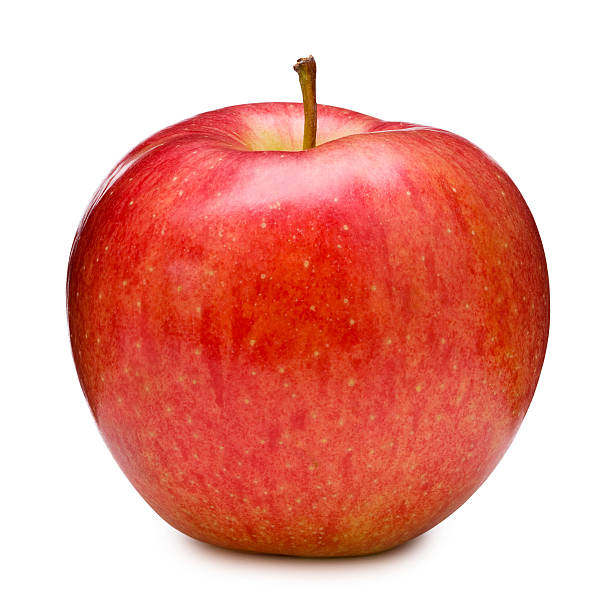
\includegraphics{images/fig1}
		\caption{My first image}
		\label{fig:1}
	\end{figure}
\end{frame}

\begin{frame}{Equations}
	\begin{equation}
	\frac{\partial y}{\partial t}=\oint\alpha\beta\sqrt{x^2+y^2} dx
	\label{My_eq}
	\end{equation}
	
	\begin{equation}
	F=am
	\label{Eq:1}
	\end{equation}
\end{frame}



\begin{frame}
	\begin{table}[h]
		\begin{center}
			\begin{tabular}{|c|c|r|c|}
				\hline
				\rule[-1ex]{0pt}{2.5ex} Name & Place & Age & Remarks \\
				\hline
				\rule[-1ex]{0pt}{2.5ex} Appu & EKM & 12 &  \\
				\hline
				\rule[-1ex]{0pt}{2.5ex} Ammu & TVM & 13 &  \\
				\hline
				\rule[-1ex]{0pt}{2.5ex} Hari & USA &12  &  \\
				\hline
				\rule[-1ex]{0pt}{2.5ex} Basi & JAP  & 7 &  \\
				\hline
				\rule[-1ex]{0pt}{2.5ex} Athul & PLUTO & 20 &  \\
				\hline
			\end{tabular}
		\end{center}
		\caption{My table}
		\label{tab:1}
	\end{table}
\end{frame}
\end{document}